\\
$g$ is a \emph{subgradient} of $f$ (not necessarily differentiable) at $x$ if
\begin{equation*}
f(y) \geq f(x) + g^T(y-x)
\end{equation*}
holds for all $y$. We write $g \in \partial f(x)$ if $g$ is a subgradient of $f$ at $x$.

\begin{center}
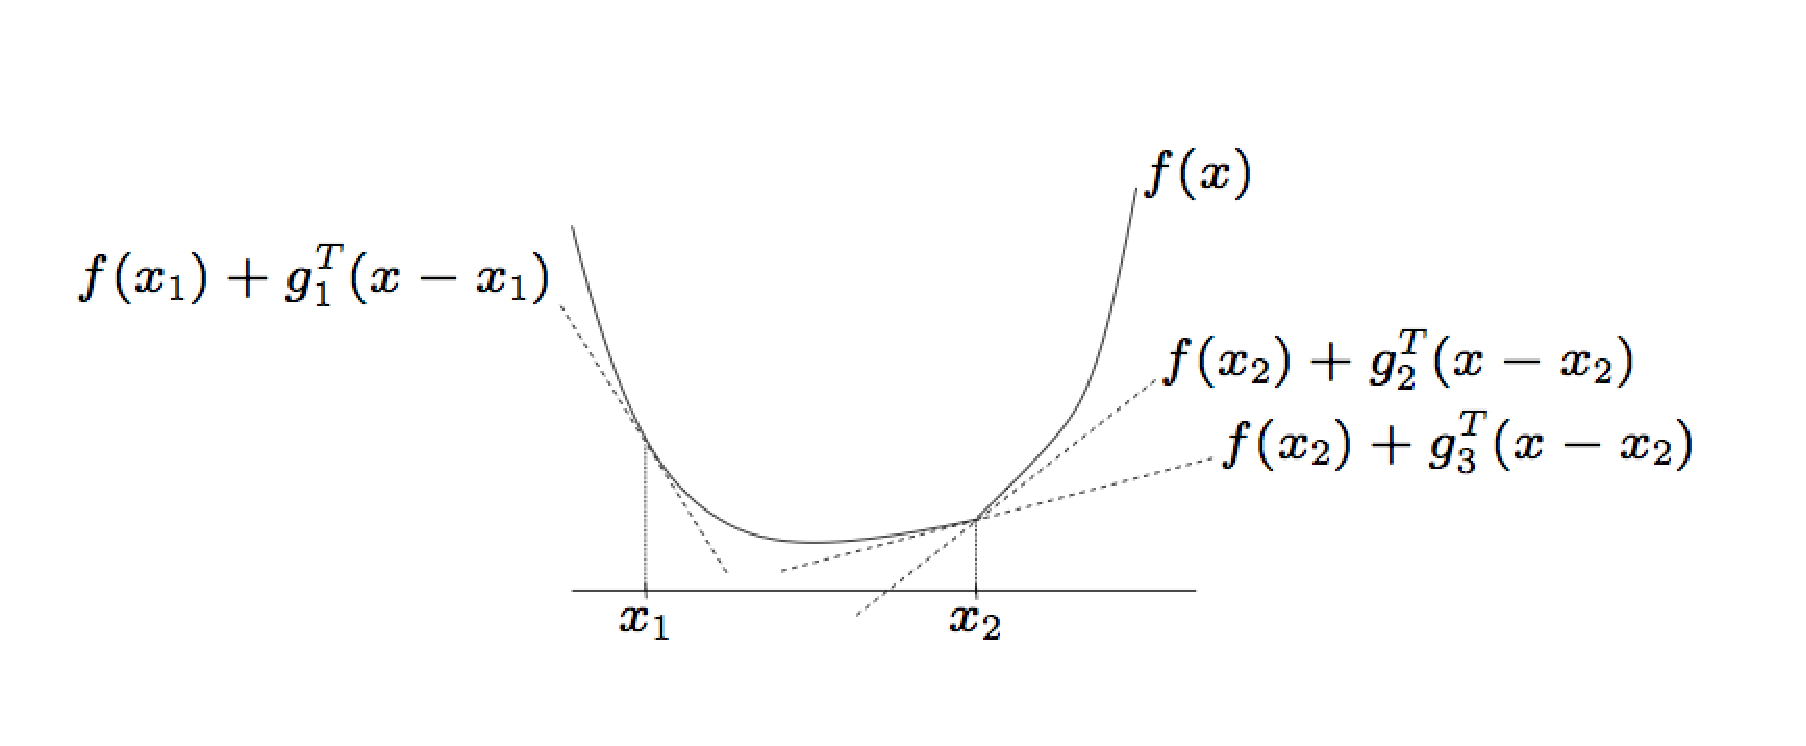
\includegraphics[width=0.95\textwidth]{poster/subgrad_figure}
\end{center}

($g_1$ is a subgradient at $x_1$. $g_2$ and $g_3$ are subgradients at
$x_2$.)